\documentclass[en]{../../../../../../eplexam}

\usepackage{../../../mmc-MECA1901-exam}

\hypertitle{Mécanique des milieux continus}{5}{MECA}{1901}{2014}{Janvier}
{Vincent Schellekens\and Antoine de Comité\and Aurélien Pignolet\and Mamadou Segpa\and Philippe Greiner}
{Philippe Chatelain et Issam Doghri}

\section{}
Interpréter le terme $\epsilon_{12}$ du tenseur des déformations. Utiliser un dessin pour votre
explication.

\begin{figure}[H]
\centering
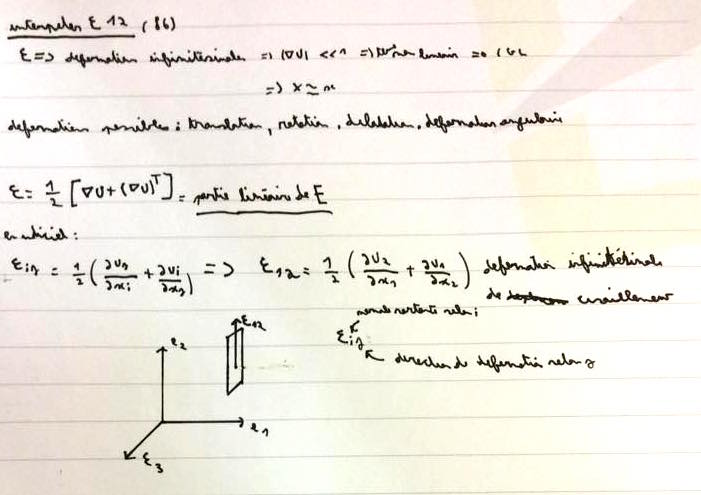
\includegraphics[scale = 0.4]{e12.jpg}
\caption{question sur epsilon 12 (pas sur)}
\end{figure}

\begin{solution}
\mypar{Complément de réponse:}

On peut également interpréter géométriquement les termes non diagonaux du tenseur de déformation - $\varepsilon_{12}$ en l'occurence. Il s'agit de la demi variation d'angle qu'a subit un angle droit situé dans le volume initial (cfr figure \ref{yoloswagderoucarnage}).
\end{solution}

\begin{figure}[H]
\centering
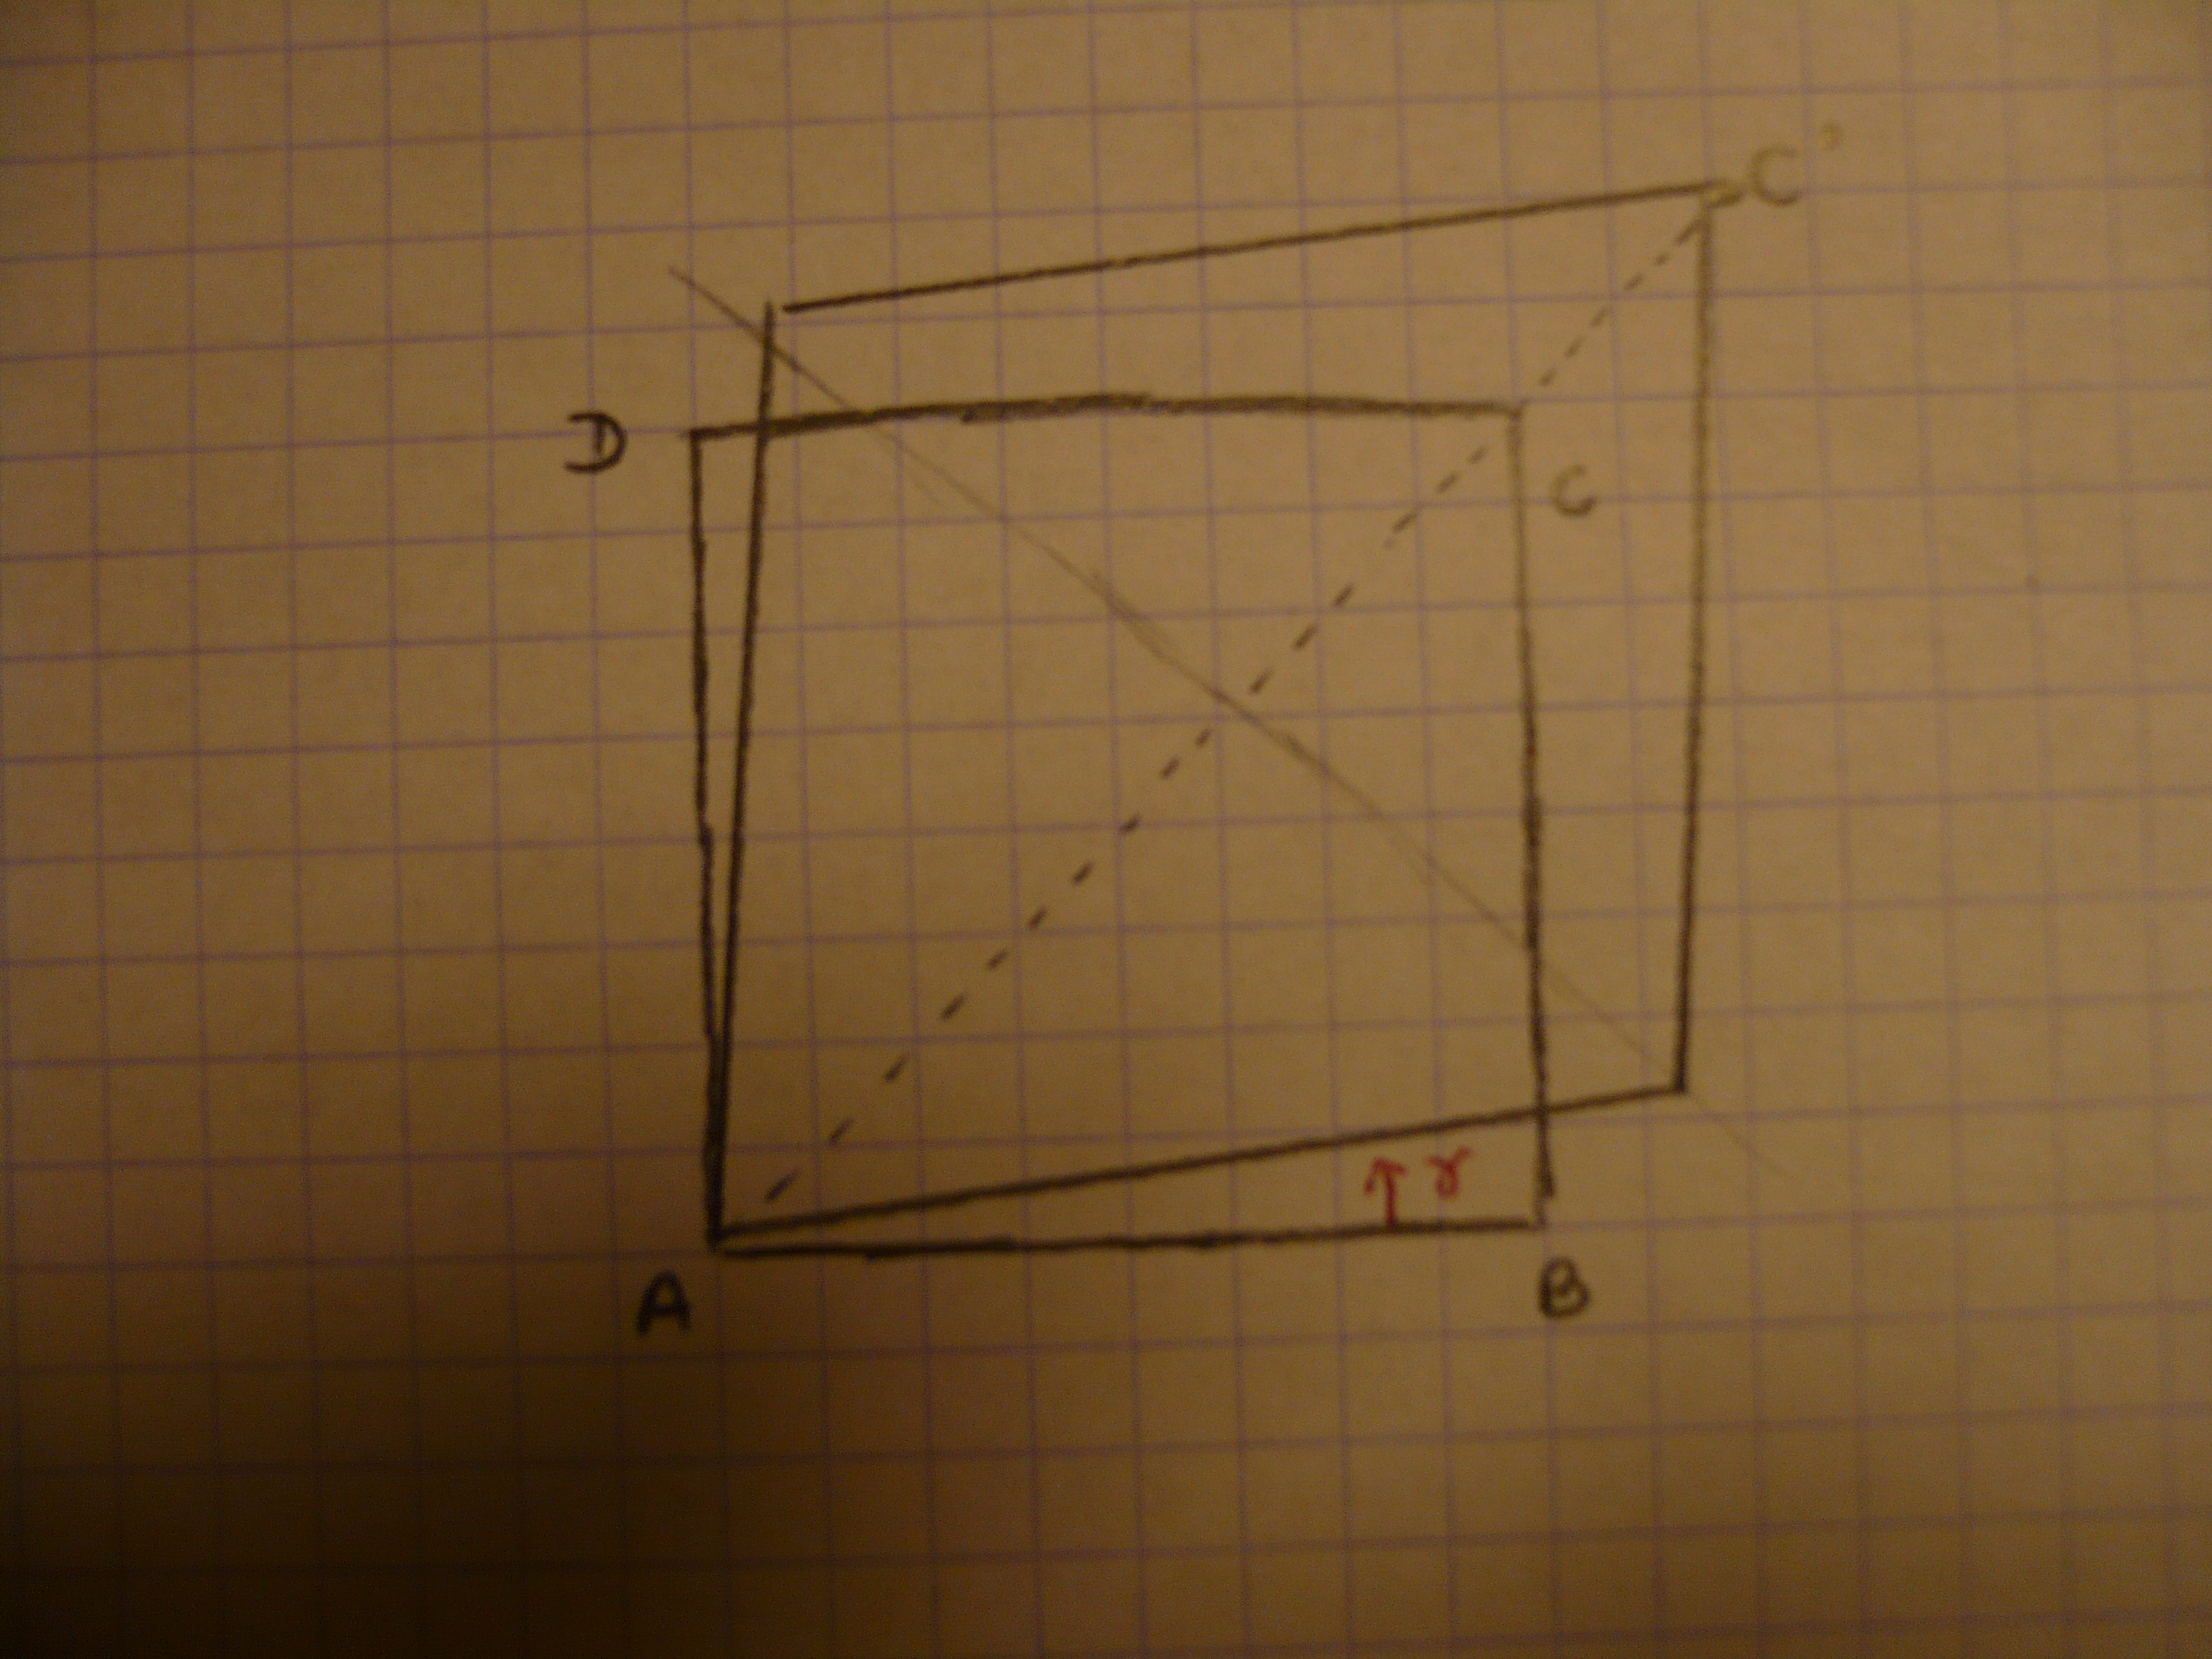
\includegraphics[width=5cm]{mignonpetitpanda.jpg}
\caption{Interprétation géométrique des termes non diagonaux}
\label{yoloswagderoucarnage}
\end{figure}


\section{}
En traction simple de valeur $\sigma$, que vaut la contrainte tangentielle maximale? Pour
répondre à la question, construisez le cercle de Mohr. Indiquez également la facette
pour laquelle la contrainte tangentielle est maximale.

\begin{figure}[H]
\centering
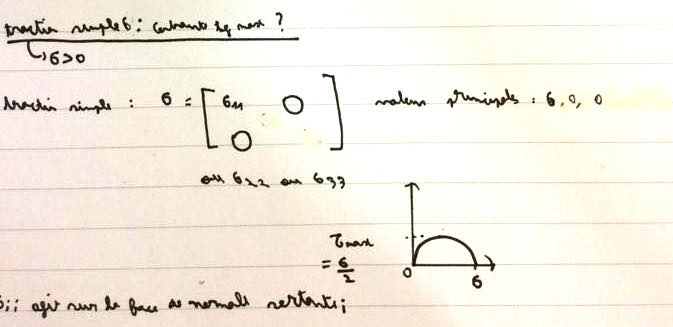
\includegraphics[scale = 0.4]{mohr.jpg}
\caption{question sur mohr (pas sur)}
\end{figure}
\begin{solution}
\mypar{Complément de réponse:}

La contrainte tangeancielle est maximale dans le plan à 45 degrés. En effet, comme il n'y a qu'un cercle de Mohr cette dernière se trouve à mi-chemin entre les deux directions principales associées au cercle.\footnote{Si il y avait trois cercles la contraintes maximale serait à 45 degrés de la contrainte maximale et minimale. Rappel: Les valeurs de $\sigma$ doivent être dans l'orde croissant}. En fait, quand on suit le contour d'un cercle de Mohr associé à deux valeurs principales, on parcourt toutes les directions entre les deux directions principales associées à ces valeurs principales. A l'apogée du cerlce on est donc parfaitement à 45 degrés des deux directions principales associées aux valeurs principales du cerlce qu'on ``suit''. %Remarque: on peut aussi trouver se plan en calculant les vecteurs propres de la matrice $det(\sigma - \lambda*I)=0$

\mypar{Autre manière de trouver la facette à force tangentielle maximale:}

En regardant le cercle de Mohr, on voit que $\tau = \tau_{max}$ quand $\sigma_n = \sigma_{11}/2$ (axe des abscisses). Si on dénote la normale à la facette à contrainte tangentielle maximale $\uline{\hat{n}} =n_i\Base{i}$, on peut calculer :

\begin{equation}
\sigma_n = (\uuline{\sigma} \cdot \uline{\hat{n}}) \cdot \uline{\hat{n}} =
\begin{bmatrix}
       \sigma_{11}  & 0 & 0 \\[0.3em]
       0            & 0 & 0 \\[0.3em]
       0            & 0 & 0
     \end{bmatrix} \cdot
     \begin{bmatrix}
       n_1  \\[0.3em]
       n_2  \\[0.3em]
       n_3
     \end{bmatrix}  \cdot
     \begin{bmatrix}
       n_1  \\[0.3em]
       n_2  \\[0.3em]
       n_3
     \end{bmatrix} = \sigma_{11} n_1^2 = \sigma_{11}/2
\end{equation}

Donc $n_1 = 1/\sqrt{2}$, et $n_2$ et $n_3$ quelquonques est la famille des normales des plans à force tangentielle maximale. On a donc bien que l'angle entre l'axe parallèle à la traction et la normale de la facette à force tangentielle vaut 45 degrés, car $\uline{\hat{n}} \cdot \Base{1} = \cos(\theta) = 1/\sqrt{2}$.
\end{solution}

\section{}
Expliquer la décomposition sphérique et déviatoire d’un tenseur. Illustrer son utilité.

\begin{solution}
Un tenseur $\uuline{A}$ peut être décomposé en une partie sphérique $\uuline{A}^{s}$, proportionnelle au tenseur unitaire $\uuline{I}$, et une partie déviatoire, $\uuline{A}^{d}$. On a donc : $\uuline{A} = \uuline{A^s} + \uuline{A}^d$.

On calcule les deux composantes comme ceci :
\begin{equation}
\uuline{A^s} = \frac{1}{3}\mathrm{Tr}\uuline{A} \uuline{I}\quad ,\quad  \uuline{A}^d = \uuline{A} - \uuline{A^s}
\end{equation}

La partie sphérique est indépendante des rotations que subit le milieu et est associée au changement de volume de celui-ci. La partie déviatoire est associée au changement de forme.

Par exemple, on peut décomposer le tenseur des contraintes $\uuline{\sigma}$ et le tenseur des déformations de Green-Lagrange $\uuline{\epsilon}$ d'un solide thermo-élastique linéaire pour obtenir l'équation de constitution suivante :

\begin{equation}
\uuline{\sigma} = \uuline{\sigma^s} + \uuline{\sigma}^d = 3 \kappa \uuline{\epsilon^s} + 2 \mu \uuline{\epsilon}^d
\end{equation}

Ou encore (1 des deux exemples suffit), on peut décomposer le tenseur des contraintes $\uuline{\sigma}$ et le tenseur des contraintes visqueuses $\uuline{\tau}$ ainsi que le tenseur des taux de déformation $\uuline{D}$ d'un fluide visqueux Newtonien pour obtenir l'équation de constitution suivante :

\begin{equation}
\uuline{\tau} = \uuline{\tau^s} + \uuline{\tau}^d = \left( \frac{2}{3}\mu + \lambda\right)\mathrm{Tr}(\uuline{D})  \uuline{I} + 2 \mu \left( \uuline{D} - \frac{1}{3}\mathrm{Tr}(\uuline{D})\uuline{I} \right)
\end{equation}

et donc comme $\uuline{\sigma} = \uuline{\tau} - p\uuline{I}$ :

\begin{equation}
\uuline{\sigma} = \uuline{\sigma^s} + \uuline{\sigma}^d = \left( \left( \frac{2}{3}\mu + \lambda\right)\mathrm{Tr}(\uuline{D}) - p \right) \uuline{I} + 2 \mu \left( \uuline{D} - \frac{1}{3}\mathrm{Tr}(\uuline{D})\uuline{I} \right)
\end{equation}


Cette écriture permet d'identifier les deux types de viscosités, à savoir la \textit{viscosité (dynamique) de cisaillement $\mu$}, associée à la partie "déviatoire", et la \textit{viscosité (dynamique) de dilation/volume $\lambda + \frac{2}{3} \mu$}, associée à la partie "sphérique".
\end{solution}

\section{}
Utiliser la loi de comportement d’un matériau hyper-élastique pour illustrer deux
principes d’établissement de lois de constitution.

\nosolution
%Je ne suis pas très sûr ici, besoin de confirmations/infiramtions

%\paragraph{Admissibilité} la loi de constitution doit respecter le second principe de la thermodynamique, via l'inégalité de Clausius-Duhem :
%\begin{equation}
%\rho T \PTDeriv{S}{T} - \rho \PTDeriv{e}{t} \geq \frac{1}{T} \textbf{q} \cdot \nabla T - \uuline{\sigma}:\uuline{D}
%\end{equation}

\section{}
Montrer que dans le cas d’un fluide visqueux newtonien incompressible et indatable,
une condition nécessaire sur l’écoulement est que son champ de vitesse soit à divergence
nulle? Pour ce cas, simplifier l’expression de la loi de constitution des contraintes.

\begin{solution}
On part de la conservation de la masse dans sa forme locale :
\begin{equation}
\PTDeriv{\rho}{t} + \rho \nabla \cdot \textbf{v} = \PDeriv{\rho}{t} + \textbf{v} \cdot \nabla \rho + \rho \nabla \cdot \textbf{v} = 0
\end{equation}

Un fluide est incompressible et indilatable quand sa masse volumique ne varie pas avec la pression (incompressible) ou avec la température (indilatable) : dès lors, on considère que la masse volumique $\rho$ est constante dans le milieu et ne dépend donc ni du temps, ni de l'espace\footnote{C'est un peu flou, les définitions sont pas vraiment claires...}. En d'autres mots, les dérivées spatiales et temporelles de $\rho$ sont nulles et on a :

\begin{equation}
\rho \nabla \cdot \textbf{v} = 0 \rightarrow \nabla \cdot \textbf{v} = 0
\end{equation}

L'équation de constitution du fluide est :
\begin{equation}
\uuline{\sigma} = 2 \mu \uuline{D} + \lambda \mathrm{Tr}(\uuline{D})\uuline{I} - p\uuline{I}
\end{equation}

On peut observer que $\mathrm{Tr}(\uuline{D}) = \PDeriv{v_i}{x_i} = \nabla \cdot \textbf{v}$, et on a alors :

\begin{equation}
\uuline{\sigma} = 2 \mu \uuline{D} - p\uuline{I}
\end{equation}

\end{solution}

\end{document}
